\documentclass[12pt]{article}  %%%,twocolumn is too scrunched. decrease margin, increase column seperation

%%% 
%%% Composition of formulas for MST Qualifying Exam
%%% All mistakes are mine, all work is cited by Author
%%% Creative Commons:
%%% Attribution-Noncommercial-Share Alike 3.0 Unported
%%% http://creativecommons.org/licenses/by-nc-sa/3.0/
%%% 

\usepackage{verbatim} %%% multi-line comments
\usepackage[pdftitle={equations for the qualifying exam}, pdfauthor={Ben Payne}, pdfsubject={equations}, pdfkeywords={maxwell, lagrange}]{hyperref}
\usepackage{times}

%%% AMS packages and font files
\usepackage{amsmath} %%% necessary for gathered equations
\usepackage{amsfonts}
%%% For figures
%%%\usepackage[dvipdfm,colorlinks=true]{hyperref}
\usepackage[dvips]{graphicx}
\usepackage[usenames,dvipsnames]{color}
\usepackage{setspace}

%%% screws up the paragraph formatting
%%%\raggedright

\begin{comment}
\setlength{\topmargin}{-.5in}
\setlength{\textheight}{9.5in}
\setlength{\oddsidemargin}{0in}
\setlength{\textwidth}{6.5in}
\end{comment}
\setlength{\topmargin}{-1in}
\setlength{\textheight}{10in}
\setlength{\oddsidemargin}{-.5in}
\setlength{\textwidth}{7.5in}


%%% Commonly used macros
%%% from https://facetsproject.org/facets/browser/trunk/docs/gsdocs/nondimtf2hall.tex
\newcommand{\pfrac}[2]{\frac{\partial #1}{\partial #2}}
\newcommand{\pfraca}[1]{\frac{\partial}{\partial #1}}
\newcommand{\pfracb}[2]{\partial #1/\partial #2}

\def\includeSchaums{T} 
\def\qualifyingyear{F}

\setlength{\columnsep}{.5in} 
\begin{document}
%%%\twocolumn
%%% or you can put it in \documentclass[11pt,twocolumn]{article}

%%% don't hyphenate so much - default = 200, max (never hyphenate) = 10,000
\hyphenpenalty=800

\title{Physics equations}
\author{Ben~Payne\footnote{Electronic address: ben.is.located@gmail.com}}
%%%\affiliation{Department~of~Physics, Missouri~University~of~Science~\&~Technology, Rolla,~MO~65409}
\date{\today}

\thispagestyle{empty}  %%% hides page number of the title page
\pagestyle{empty} %%% no page numbers on the following pages
%%%\begin{abstract}
%%%equations for the qualifying exam
%%%\end{abstract}

version 0.64, 20090308

%%% http://clarku.edu/~djoyce/trig/identities.html
\if\includeSchaums T
%%%%%%%%%%%%%%%%%%%%%%%%%%%%%%%%%%%%%%%%%%%%%%%%%%%%%%%%%%%%%%%%%%%%%%%%%%%%%
\section{coordinate systems}
%%%%%%%%%%%%%%%%%%%%%%%%%%%%%%%%%%%%%%%%%%%%%%%%%%%%%%%%%%%%%%%%%%%%%%%%%%%%%
(from cover of \cite{GriffithED}.) Most can be found in Schaum's.
%%%\begin{comment}
 the following is in Schaum's, pg 120
\subsection{cartesian}
%%%\Huge
\begin{equation}
dV = 	dx\cdot dy\cdot dz
\label{eq:cartesian_dV}
\end{equation}
%%%\normalsize
gradient: 
%%%\Huge
\begin{equation}
\vec{\nabla} t = \widehat{x} \pfrac{t}{x}  + \widehat{y} \pfrac{t}{y} + \widehat{z} \pfrac{t}{z}  %%% can't seem to get \hat to work
\label{eq:cartesian_gradient}
\end{equation}
%%%\normalsize
divergence (equ 1.40, page 17 \cite{GriffithED})
%%%\Huge
\begin{equation}
 \vec{\nabla} \cdot v = \pfrac{v_x}{x} + \pfrac{v_y}{y} + \pfrac{v_z}{z}
\label{eq:cartesian_divergence}
\end{equation}
%%%\normalsize
laplacian
\begin{equation}
\nabla^2 f = \pfrac{^2 f}{x^2} + \pfrac{^2 f}{y^2} + \pfrac{^2 f}{z^2}
\label{eq:cartesian_laplacian}
\end{equation}
%%%\end{comment}
%%%%%%%%%%%%%%%%%%%%%%%%%%%%%%%%%%%%%%%%%%%%%%%%%%%%%%%%%%%%%%%%%%%%%%%%%%%%%
\subsection{spherical}

\begin{equation}
dV = 	r^2 \ \sin \theta \ dr \ d\theta \ d\phi
\label{eq:spherical_dV}
\end{equation}

page 40, \cite{GriffithED}
\begin{equation}
  d \vec{a} = \hat{r} \ r^2 \sin \theta \ d\theta \ d\phi
\end{equation}

\begin{equation}
\vec{\nabla} = \hat{r}\pfraca{r}+ \hat{\theta}\frac{1}{r}\pfraca{\theta}+\hat{\phi}\frac{1}{r\sin\theta}\pfraca{\phi}
\label{eq:spherical_gradient}
\end{equation}

%%%\begin{comment}
 Schaum's, pg 126
laplacian. See \htmladdnormallink{planetMath laplacian rectangualr to cartesian}{http://planetmath.org/encyclopedia/DerivationOfTheLaplacianFromRectangularToSphericalCoordinates.html}
and \htmladdnormallink{planetMath laplacian}{http://planetmath.org/?method=l2h&from=collab&id=76&op=getobj}
(equ 3.53, page 137 \cite{GriffithED})
\begin{equation}
\nabla^2 f = {1 \over r^2} {\partial \over \partial r}  \left( r^2 {\partial f \over \partial r} \right) 
+ {1 \over r^2 \sin \theta} {\partial \over \partial \theta}  \left( \sin \theta {\partial f \over \partial \theta} \right) 
+ {1 \over r^2 \sin^2 \theta} {\partial^2 f \over \partial \phi^2}
\label{eq:spherical_laplacian}
\end{equation}
%%%\end{comment}

%%%%%%%%%%%%%%%%%%%%%%%%%%%%%%%%%%%%%%%%%%%%%%%%%%%%%%%%%%%%%%%%%%%%%%%%%%%%%
\subsection{cylindrical}

\begin{equation}
dV = 	s \ ds \ d\phi \ d\theta
\label{eq:cylindrical_dV}
\end{equation}

\begin{equation}
\vec{\nabla} = \hat{s}\pfraca{s} + \hat{\phi}\frac{1}{s} \pfraca{\phi} + \hat{z}\pfraca{a}
\label{eq:cylindrical_gradient}
\end{equation}

%%%\begin{comment}
\begin{equation}
\nabla^2 f = {1 \over \rho} {\partial \over \partial \rho}  \left( \rho {\partial f \over \partial \rho} \right) 
+ {1 \over \rho^2} {\partial^2 f \over \partial \theta^2} + {\partial^2 f \over \partial z^2 }
\label{eq:cylindrical_laplacian}
\end{equation}
%%%\end{comment}
\fi
\section{formulas}

material in this section can NOT be found in Schaum's \htmladdnormallink{mathematical handbook of formulas}{http://site.ebrary.com/lib/umr/Doc?id=10015341}, which is allowed on the day of the exam.
%%%\begin{comment}
 Schaum's, 123 \\ 
Stoke's thm (equ 1.57, page 34 \cite{GriffithED})
\begin{equation}
\int_{surface} (\vec{\nabla}\cdot\vec{v})\cdot d\vec{a} = \oint_{volume}\vec{v}\cdot d\vec{l}
\label{eq:stokesThm}
\end{equation}
%%%\end{comment}

Greene's thm (equ 1.56, page 31 \cite{GriffithED})
\begin{equation}
\int_{volume}(\vec{\nabla}\cdot\vec{v}) d\tau = \oint_{surface} \vec{v}\cdot d\vec{a}
\label{eq:greenesThm}
\end{equation}

Taylor series expansion is in Schaum's, but the easy approximation is not. (assuming small x)
\begin{equation}
(1+x)^n \approx 1 + n x
\label{eq:TaylorSeriesApprox}
\end{equation}

%%%\begin{comment}
 in Schuam's \\ 
Taylor series expansion
%%% \begin{widetext} %%% not recognized
%%%\begin{multicols}{2}%%% not recognized
\begin{equation}
f(x) = f(a) + f'(x)|_a (x-a) + \frac{1}{2!} f''(x)|_a (x-a)^2 + \cdots
\label{eq:TaylorSeries}
\end{equation}
%%%\end{multicols}%%% not recognized
%%%\end{widetext} %%% not recognized
%%%\end{comment}


\section{Math}
\begin{equation}
\left[ \begin{array}{cc}
  \cos \theta & \sin \theta \\
-\sin \theta  & \cos \theta \\
 \end{array} \right]
\left[ \begin{array}{c}
A_x\\
A_y
\end{array}\right]
=
\left[ \begin{array}{c}
A_{x'}\\
A_{y'}
\end{array}\right]
\end{equation}
\begin{center}
 \includegraphics[scale=0.3]{pictures/coordinate_rotation}
\end{center}


Variance
\begin{equation}
(\Delta A)^2 = \langle A^2 \rangle - \langle A \rangle^2 
\end{equation}

Quadratic equation
\begin{equation}
 x = \frac{-b \pm \sqrt{b^2 - 4ac}}{2a}
\end{equation}


%%%%%%%%%%%%%%%%%%%%%%%%%%%%%%%%%%%%%%%%%%%%%%%%%%%%%%%%%%%%%%%%%%%%%%%%%%%%%
\section{Electromagnetics} %%
%%%%%%%%%%%%%%%%%%%%%%%%%%%%%%%%%%%%%%%%%%%%%%%%%%%%%%%%%%%%%%%%%%%%%%%%%%%%%

%%%%%%%%%%%%%%%%%%%%%%%%%%%%%%%%%%%%%%%%%%%%%%%%%%%%%%%%%%%%%%%%%%%%%%%%%%%%%
\subsection{Maxwell equations} %%
%%%%%%%%%%%%%%%%%%%%%%%%%%%
%%% see http://hyperphysics.phy-astr.gsu.edu/HBASE/electric/maxeq.html
See also page 22, \cite{ReifThermo}; page 2, \cite{JacksonED} \\ 
%%%\begin{align} %%% utilizes the "&"
\underline{Faraday}'s law (equation 7.16, page 302, \cite{GriffithED})
\begin{equation}
  \vec{\nabla}\times \vec{E} = -\pfrac{\vec{B}}{t} 
  \label{eq:maxwellEcurl}
\end{equation}

\underline{Ampere}'s law (equation 5.54, page 225 and equation 5.44, page 222 \cite{GriffithED})
\begin{equation}
  \vec{\nabla}\times \vec{B} =  \mu_0\vec{J}+\frac{1}{c^2}\pfrac{\vec{E}}{t} 
  \label{eq:maxwellBcurl}
\end{equation}
where
\begin{equation}
 c = \frac{1}{\sqrt{\epsilon_0 \mu_0}}
\end{equation}

\underline{Gauss}'s law, electricity (equation 2.14, page 69 \cite{GriffithED})
\begin{equation}
  \vec{\nabla}\cdot\vec{E} = \frac{\rho}{\varepsilon_0} 
  \label{eq:maxwellEdiv} 
\end{equation}

\underline{Guass}'s law, magnetism (equation 5.48, page 223 \cite{GriffithED})
\begin{equation}
  \vec{\nabla}\cdot\vec{B} = 0  
  \label{eq:maxwellBdiv}
\end{equation}
%%%\end{align}
Integral forms:

flux of electric field (equation 2.11, page 67 \cite{GriffithED})
\begin{equation}
\Phi_E = \int_{any\ surface} \vec{E} \cdot d\vec{a}
\end{equation}

\underline{Gauss}'s law, electricity. (equation 2.13, page 68 \cite{GriffithED})
\begin{equation}
  \oint_{closed\ surface} \vec{E}\cdot d\vec{a} = \frac{Q_{enclosed}}{\epsilon_0}
	\label{eq:GaussLaw}
\end{equation}

\underline{Faraday}'s Law (equation 7.18, page 306 \cite{GriffithED}) 
\if\qualifyingyear T
(2008 A3)
\fi
\begin{equation}
  \oint \vec{E} \cdot d\vec{l} = - \frac{d\Phi _B}{dt}
	\label{eq:Faraday_law}
\end{equation}

\underline{Ampere}'s law (equation 5.55, page 225 and 5.42, page 222 \cite{GriffithED}) 
\if\qualifyingyear T
(2008 A3)
\fi
\begin{equation}
  \oint \vec{B} \cdot d\vec{l} = \mu_0 I_{enclosed}
	\label{eq:Ampere}
\end{equation}

\underline{Ampere}'s law (page 306, \cite{GriffithED})
\begin{equation}
  \oint \vec{B} \cdot d\vec{l} = \mu_0 I_{enclosed} + \mu_0 \epsilon_0 \int \left( \frac{d}{dt}\vec{E}\right) \cdot d\vec{a}
	\label{eq:Ampere_large}
\end{equation}

\underline{Lorentz} force law (equation 5.2, page 204 \cite{GriffithED}). Also equation 1-61, page 22 \cite{GoldsteinCM}
\begin{equation}
\vec{F} = q (\vec{E} + \vec{v}\times \vec{B})
\end{equation}

%%%%%%%%%%%%%%%%%%%%%% end maxwell %%%%%%%%%%
\subsection{general EM}
%%%%%%%%%%%%%%%%%%%%%%%%%%%%%%%%%%%%%%%%%%%%%%

equation 1-62, page 22 \cite{GoldsteinCM}
\begin{equation}
\vec{B} = \vec{\nabla} \times \vec{A}
\end{equation}

Coulomb's Law
\begin{equation}
\vec{F} =\frac{1}{4\pi \epsilon _{0} } \frac{q_{1} q_{2} }{r^{2} } \hat{r}
\end{equation}
 where $q_{2} $ is the test charge

\begin{equation}
\vec{E}=\frac{1}{4\pi \epsilon_0} \int_v \frac{\rho}{r^2} d \tau \hat{r}
\end{equation}

electric displacement (see also eq \ref{eq:electricDisplacementwithPolarization})
\begin{equation}
\vec{D} = \epsilon_0 \vec{E}
	\label{eq:electricDisplacement}
\end{equation}

Electric field due to point charge (equation 2.4, page 60 \cite{GriffithED})
\begin{equation}
\vec{E} = \frac{1}{4 \pi \epsilon_0} \sum_i \frac{q_i}{r_i^2} \hat{r}_i
%%%\label{eq:another}
\end{equation}


electrostatic potential (equ 2.21, page 78 and equ 7.10, page 293\cite{GriffithED})
\begin{equation}
V = - \int^r_{\infty} \vec{E}\cdot d\vec{l}
%%%\label{eq:another}
\end{equation}

electric field and electrostatic potential (equation 2.23, page 78,  \cite{GriffithED})
\begin{equation}
  \vec{E} = -\vec{\nabla}V
	\label{eq:electric_field_potential}
\end{equation}

electrostatic potential (equation 2.27, page 84 \cite{GriffithED})
\begin{equation}
 V = \frac{1}{4 \pi \epsilon_0} \sum_i \frac{q_i}{r_i}
\end{equation}

electrostatic potential (equation 2.29, page 84 \cite{GriffithED})
\begin{equation}
 V = \frac{1}{4 \pi \epsilon_0} \int \frac{\rho}{r} d \tau
\end{equation}

work (equation 2.42, page 92  \cite{GriffithED})
\begin{equation}
  W = \frac{1}{2} \sum q_i V(r_i)
%%%\label{eq:}
\end{equation}

work and electrostatic potential (equ 2.45, page 94 \cite{GriffithED})
\begin{equation}
  W = \frac{\epsilon_0}{2} \int_{all space} E^2 d \tau
\label{eq:work_in_electric_field}
\end{equation}

surface charge density and electrostatic potential (where $n$ is the normal direction \\ (equation 2.49, page 102  \cite{GriffithED})
\begin{equation}
\sigma = -\epsilon_0 \frac{\partial V}{\partial n}
\label{eq:surfacechargedensity}
\end{equation}

equation 2.48, page 102 \cite{GriffithED}
\begin{equation}
\vec{E} = \frac{\sigma}{\epsilon} \hat{n}
\end{equation}


electric displacement, including polarization (equ 4.21, page 175 \cite{GriffithED})
(see also eq \ref{eq:electricDisplacement})
\begin{equation}
\vec{D} = \epsilon_0 \vec{E} + \vec{P}
\label{eq:electricDisplacementwithPolarization}
\end{equation}

work and electrostatic potential (equ 2.55, page 106, \cite{GriffithED})
\begin{equation}
  W = \frac{1}{2} C V^2
	\label{eq:workCapacitor}
\end{equation}

electrostatic potential due to a monopole (equation 3.97, page 149  \cite{GriffithED})
\begin{equation}
V_{monopole} = \frac{1}{4 \pi \epsilon_0} \frac{Q}{r}
\end{equation}

electrostatic potential due to a dipole (equation 3.99, page 149  \cite{GriffithED})
\begin{equation}
V_{dipole} = \frac{1}{4 \pi \epsilon_0} \frac{\vec{p}\cdot \hat{r}}{r^2}
\end{equation}

where dipole moment (which points from the (-) charge to the (+) is \\ 
(equation 3.98, page 149  \cite{GriffithED}) (equation 3.100, page 150  \cite{GriffithED})
\begin{equation}
\vec{p} = \int \vec{r} \; ' \rho ( \vec{r}\;' ) d \tau \;' = \sum_i q_i r_i
\end{equation}

Note: $E_{dipole}$, equation 3.104, page 155; is given on 2002 B10,
but as a derivation (see also problem 3.33).

Torque ($N$) is on a dipole ($\vec{p}=q\vec{d}$) due to E field (equation 4.4, page 164, \cite{GriffithED})
\begin{equation}
\vec{N} = \vec{p} \times \vec{E}
\end{equation}

potential energy of a dipole (problem 4.7) (equation 4.6, page 165, \cite{GriffithED})
\begin{equation}
U = -\vec{p} \cdot \vec{E}
\end{equation}

Similarly for magnetic moment ($\vec{\mu} = (\vec{I} \cdot \vec{A})\hat{n}$) \\ 
(equation 6.1, page 257, \cite{GriffithED}) 
\begin{equation}
\vec{N} = \vec{\mu} \times \vec{B} \\ 
\end{equation}

potential energy (equation 6.34, page 281, \cite{GriffithED}) 
\begin{equation}
U = -\vec{\mu} \cdot \vec{B}
\end{equation}

force due to magnetic field (equ 5.16, page 205 \cite{GriffithED})
\if\qualifyingyear T
(1997 A4)
\fi
\begin{equation}
 F_{magnetic} = I \int d\vec{l} \times \vec{B}
\end{equation}

(equ 6.31, page 275 \cite{GriffithED})
\begin{equation}
 \vec{B} = \mu \vec{H}
\end{equation}

(equ 6.32, page 275 \cite{GriffithED}) 
\if\qualifyingyear T
(2009 A)
\fi
\begin{equation}
 \mu = \mu_0 (1+\chi_m)
\end{equation}

(equ 7.3, page 285 \cite{GriffithED})
\begin{equation}
 \vec{J} = \sigma \vec{E}
\end{equation}

flux (equ 7.12, page 295 \cite{GriffithED}) 
\if\qualifyingyear T
(1997 A4, 2009 A)
\fi
\begin{equation}
 \Phi = \int \vec{B} \cdot d\vec{a}
\end{equation}

work (equ 7.29, page 317 \cite{GriffithED}). Used in problems 7.26, 7.27. 
\if\qualifyingyear T
(2008 A3)
\fi
\begin{equation}
  W = \frac{1}{2} L I^2
	\label{eq:work_self_inductance}
\end{equation}

work (equ 7.34, page 317 \cite{GriffithED}) 
\if\qualifyingyear T
(2009 A)
\fi
\begin{equation}
  W = \frac{1}{2 \mu_0} \int_{all space} B^2 d \tau
	\label{eq:work_in_magnetic_field}
\end{equation}

flux, inductance (equ 7.25, page 313 \cite{GriffithED})
\if\qualifyingyear T
(2009 A)
\fi
\begin{equation}
 \Phi = L I
\end{equation}


Power (equ 8.11, page 347 \cite{GriffithED}), positive on page 349
\begin{equation}
  Power = \int \vec{S} \cdot d\vec{a}
	\label{eq:power_fields}
\end{equation}

total potential energy in a field (equation 8.5, page 346 \cite{GriffithED}) (combines \ref{eq:work_in_magnetic_field} and \ref{eq:work_in_electric_field})
\begin{equation}
U_{em} = \frac{1}{2} \int ( \epsilon_0 E^2 + \frac{1}{\mu_0} B^2 ) d \tau
\end{equation}


Poynting vector (equation 8.10, page 347 \cite{GriffithED})
\begin{equation}
  \vec{S} = \frac{1}{\mu} \vec{E}\times\vec{B}
	\label{eq:Poynting_vector}
\end{equation}

Power and Poynting vector (equation 8.11, page 347 \cite{GriffithED})
\begin{equation}
P = \frac{dW}{dt} = - \frac{dU_{em}}{dt}- \oint \vec{S} \cdot d\vec{a}
\end{equation}

\subsection{circuits}

capacitance (equ 2.53, page 104, \cite{GriffithED})
\begin{equation}
  C \equiv \frac{Q}{V}
\end{equation}

\begin{equation}
 P=I^2 R
\end{equation}

\begin{equation}
 V=IR
\end{equation}


Power and electrostatic potential ($P=I^2 R$ can be derived from $V=IR$) \\ 
(equation 7.7, page 290, \cite{GriffithED})
\begin{equation}
  Power = I V
	\label{eq:power_current}
\end{equation}

circuit sum (equation 7.4, page 290, \cite{GriffithED}) [resistor, capacitor, inductor]
\begin{equation}
V = IR + \frac{Q}{C} + L \frac{dI}{dt}
\end{equation}
 \begin{center}
  \includegraphics[scale=0.3]{pictures/V_R_C_L}
 \end{center}

\begin{equation}
I = \frac{dQ}{dt}
\end{equation}

capacitance, A is the area, d is the seperation (equation 2.54, page 105 \cite{GriffithED})
\begin{equation}
C = \frac{A \epsilon_0}{d}
\end{equation}


%%%%%%%%%%%%%%%%%%%%%%%%%%%%%%%%%%%%%%%%%%%%%%%%%%%%%%%%%%%%%%%%%%%%%%%%%%%%%
\subsection{relativity}

Lorentz factor, [$\gamma > 1$](equation 12.6, page 486 \cite{GriffithED})
\begin{equation}
\gamma = \frac{1}{\sqrt{1-(\frac{v}{c})^2}}
\label{eq:gamma}
\end{equation}
\if\qualifyingyear T
GIVEN on 2008 A1, not given on 2001 A6\\ 
\fi
 total relativistic energy for free particle (equation 12.55, page 551 \cite{GriffithED})
\begin{equation}
  E = \sqrt{m^2 c^4 + p^2 c^2}
	\label{eq:relativistic_energy}
\end{equation}

\begin{equation}
  E = \gamma m c^2
	\label{eq:Einsteins_energy}
\end{equation}


relativistic momentum (equation 2-7, page 71 \cite{TiplerMP}) 
\if\qualifyingyear T
\\ 
2001 A5 d
\fi
\begin{equation}
  p = \gamma m v
  \label{eq:relativistic_momentum}
\end{equation}

\subsection{EM concepts}
\begin{itemize}
	\item hollow charged conductors have no interior electric field (page 97, \cite{GriffithED})
	\item solid evenly-charged spheres have linearly increasing electric field inside;
	outside E field falls of as $\frac{1}{r^2}$
	\item potential of a charge falls off as $\frac{1}{r}$
	\item length contraction, time dilations (chapter 12, \cite{GriffithED})
	\item images above an $\infty$ grounded conducting plane $\rightarrow$ use method of images 
	(section 3.2, see also problem 4.6 in \cite{GriffithED})
	\item changing electric field induces a magnetic field (page 323, \cite{GriffithED})
	\item magnetic forces do no work (page 207, \cite{GriffithED})
	\item $E_{tangential}$ is continuous, $E_{normal}$ is discontinuous
	\item to solve Laplace's equation ($\nabla^2 V = 0$) with V specified on the
	boundaries, use seperation of variables (Chapter 3, \cite{GriffithED})
	\item magnetic forces do no work (page 207, \cite{GriffithED})
\end{itemize}

%%%%%%%%%%%%%%%%%%%%%%%%%%%%%%%%%%%%%%%%%%%%%%%%%%%%%%%%%%%%%%%%%%%%%%
\section{Thermodynamics}
%%%%%%%%%%%%%%%%%%%%%%%%%%%%%%%%%%%%%%%%%%%%%%%%%%%%%%%%%%%%%%%%%%%%%%
most generally, specific heat is 
\begin{equation}
C_x = \frac{dQ}{dT}|_x
\end{equation}
where x is the variable that is held constant. 
\begin{equation}
 \frac{1}{T} = \pfrac{S}{E} |_v
\end{equation}
Then from equation  $5 \cdot 6 \cdot 1$ page 164; page 153; \cite{ReifThermo}
\begin{equation}
T \cdot dS = dE + p \cdot dV
\label{eq:TdS}
\end{equation}
solve for $dE$, which is $dQ$, and hold V constant to get \\ 
specific heat, constant volume; 
\if\qualifyingyear T
given on 2002 A6
\fi
\begin{equation}
C_V = \pfrac{E}{T}|_v
\end{equation}
using the definition of enthalpy, add $d(pV)$ to Eq.~\ref{eq:TdS} to get
\begin{equation}
dH = T \cdot dS + V \cdot dp
\end{equation}
and hold pressure p constant to get \\ 
specific heat, constant pressure
\begin{equation}
C_p = \pfrac{H}{T}|_p
\end{equation}
\begin{equation}
 C_P = C_V + N K_{Boltzmann} = C_V + \nu R
\end{equation}
$C_P > C_V$ always
\begin{equation}
 pV = \nu R T
\end{equation}
where $\nu$ is the number of moles, $\frac{N}{N_{Av}}$ and $R=N_{Av} K_{Boltzmann}$.

equations $3 \cdot 3 \cdot 12$; $3 \cdot 11 \cdot 6$, page 123; \cite{ReifThermo}
\if\qualifyingyear T
 \\ 
given on 2002 B6, 2006 A6
\fi
\begin{equation}
S = k \ln \Omega
\end{equation}

ideal gas; relating average pressure, Volume, Temperature (equations  $3 \cdot 12 \cdot 8$ page 125; $7 \cdot 2 \cdot 8$ page 241; \cite{ReifThermo})
\begin{equation}
\overline{p} V = N k_{Boltzmann} T
\end{equation}
$pV = nRT$ \\ 
ideal gas; relating to average Kinetic energy
\begin{equation}
\overline{p} V = \frac{2}{3} N \overline{K}
\end{equation}

where number density $ n = \frac{N}{V}$ is number of molecules per volume. 

mean kinetic energy per particle; applies to fluids in closed systems
\begin{equation}
\overline{K} = \frac{3}{2} k_{boltzmann} T
\end{equation}

partition function for a single particle (equation $6 \cdot 5 \cdot 3$ page 213; \cite{ReifThermo}) 
\if\qualifyingyear T
\\ 
given 2002 A6
\fi
\begin{equation}
z \equiv \sum_r^\infty e^{-\beta E_r}
\end{equation}
and total partition function $Z = z^{3N}$ \\ 
partition function and energy (equation $6 \cdot 5 \cdot 4$ page 213; \cite{ReifThermo})
\if\qualifyingyear T
\\ 
given 2002 A6
\fi
\begin{equation}
E = - \frac{\partial (\ln Z)}{\partial \beta} |_V
\end{equation}

Fermi-Dirac distribution  (equation $9 \cdot 3 \cdot 14$ page 341; \cite{ReifThermo}) \\ 
mean occupation number; number of particles with energy $\epsilon_s$
\begin{equation}
n = \frac{1}{e^{\alpha + \beta \epsilon_s} +1}
\end{equation}

Bose-Einstein distribution  (equation $9 \cdot 3 \cdot 22$ page 342; \cite{ReifThermo})
\begin{equation}
n = \frac{1}{e^{\alpha + \beta \epsilon_s}-1} 
\end{equation}
since when the exponent is 0, then $n \rightarrow \infty$, so all the particles form a BEC.\\ 
Maxwell-Boltzmann distribution  (equation $9 \cdot 4 \cdot 7$ page 345; \cite{ReifThermo})
(see also page 133, \cite{TiplerMP})
\begin{equation}
n = N \frac{ e^{-\beta \epsilon_s }}{ \sum_r e^{-\beta \epsilon_r} }
\end{equation}

\subsection{Thermodynamics concepts}
\begin{itemize}
	\item good review of basics on page 122 of \cite{ReifThermo}, including the laws 
	\item second law: $\Delta S \geq 0$
	\item classical equipartition theorm: each squared term of the Hamiltonian
	has $E=\frac{1}{2}k_b T$ \\ (equation $7 \cdot 5 \cdot 7$ page 249; \cite{ReifThermo})
	\item entropy is maximum for a closed, isolated system at equilibrium
	\item all states are equally probable. Equilibrium is the most probable configuration -- the largest number of states sharing the same configuration
\end{itemize}

%%%%%%%%%%%%%%%%%%%%%%%%%%%%%%%%%%%%%%%%%%%%%%%%%%%%%%%%%%%%%%%%%%%%%%
\section{Classical Mechanics}
%%%%%%%%%%%%%%%%%%%%%%%%%%%%%%%%%%%%%%%%%%%%%%%%%%%%%%%%%%%%%%%%%%%%%%
the ``basics:'' \\ 
Force and potential energy, (page 20, \cite{GoldsteinCM})
\begin{equation}
\vec{F} = - \vec{\nabla} V
\end{equation}
\begin{equation}
 T = \frac{1}{2} I \omega^2
\end{equation}

for circular motion, tangential velocity is
\begin{equation}
v = \omega r
\end{equation}
and centripital acceleration (also circular motion)
\if\qualifyingyear T
(2009 A)
\fi
\begin{equation}
\frac{v^2}{R}
\end{equation}

Angular momentum $\vec{L}$
\begin{equation}
\vec{L} = \vec{r} \times \vec{p}
\end{equation}

Torque $\vec{N}$
\begin{equation}
 \vec{N} = \vec{r}\times \vec{F} = \pfrac{\vec{L}}{t}
\end{equation}

Force $F$, potential $V$, momentum $p$
\begin{equation}
 \vec{F} = -\vec{\nabla} V = \pfrac{p}{t}
\end{equation}

\begin{equation}
\begin{gathered}
F_{spring} = -k \ x \\ 
V_{spring} = \frac{1}{2}k \ x^2
\end{gathered}
\end{equation}

\subsection{Lagrange's Equations of Motion}

kinetic energy (cartesian, cylindrical)
\begin{equation}
T = \frac{1}{2} m v^2 = \frac{1}{2} m ( \dot{x}^2 + \dot{y}^2 + \dot{z}^2) = 
\frac{1}{2} m (\dot{r}^2 + r^2 \dot{\theta}^2 + \dot{z}^2)
\end{equation}

Lagrangian
$L=L\left( q_{j} ,\dot{q} _{j} ,t\right) =T-U$ (equation 1-56, page 20 \cite{GoldsteinCM}). \\ 
(equation 1-57, page 21 \cite{GoldsteinCM})
\if\qualifyingyear T
(2009 A)
\fi
\begin{equation}
\frac{d}{dt} \left( \frac{\partial L}{\partial \dot{q} _{j} } \right) -\frac{\partial L}{\partial q_{j} } = 0
\end{equation}

\subsection{Hamilton's Equations of Motion}
$H=H\left( q_{j} ,p_{j} ,t\right) $ \\ 
usually $ H = T+V$ \\ 
(equation 8-8, page 341 \cite{GoldsteinCM})
\begin{equation}
H=\sum\limits_{j}p_{j}  \dot{q} _{j} -L
\end{equation}

Once Lagrangian is found, get canonical momentum
\begin{equation}
p_j \equiv \frac{\partial L}{\partial \dot{q}_j }
\label{eq:canonical_momentum}
\end{equation}

and solve for $\dot{q}_j$ for later

\begin{equation}
h = \left( \sum \dot{q_j} \frac{\partial L}{\partial \dot{q} _{j} } \right) - L
\end{equation}

then substitue in $\dot{q}$ to get H. \\ 
Finally, get Hamilton Equations of motion by \\ 
(equation 8-12, page 342 \cite{GoldsteinCM})
\begin{equation}
\begin{gathered}
\dot{q} _{j} =\frac{\partial H}{\partial p_{j} } \\ 
\dot{p} _{j} = - \left( \frac{\partial H}{\partial q_{j} } \right) 
\end{gathered}
\end{equation}

then integrate to get $q$ and $p$

\subsection{2-body central force}
standard orbit is Counter Clock-Wise (CCW). \\ 
Given the Lagrangian in polar coordinates, one derives the canonical angular momentum \\ 
(equation 3-8, page 73 \cite{GoldsteinCM}) (see eq \ref{eq:canonical_momentum})
\begin{equation}
l = \mu r^2 \dot{\theta}
\end{equation}
for perturbed orbits, $ \tau > \tau_c$ implies CCW (positive $\Delta\theta$) motion (forward orbital motion)
\begin{equation}
\Delta \theta = \frac{l}{m r^2}(\tau - \tau_c)
\end{equation}

circular orbit condition (equation 3-12, page 74  \cite{GoldsteinCM})
\begin{equation}
f^{effective}(r_c) = 0 = f(r_c) + \frac{l^2}{\mu r_c^3}
\end{equation}
where for the kepler problem $f(r) = -\frac{k}{r^2}$

small oscillations of orbit
\if\qualifyingyear T
(2009 A)
\fi
\begin{equation}
r = r_c + \epsilon
\end{equation}

not included: small oscillation (chapter 6 of  \cite{GoldsteinCM}).


%%%%%%%%%%%%%%%%%%%%%%%%%%%%%%%%%%%%%%%%%%%%%%%%%%%%%%%%%%%%%%%%%%%%%%%%%%%%%
\section{Quantum}

expectation value, average, mean
\begin{equation}
\langle A \rangle = \langle \psi | A | \psi \rangle = \int_{-\infty}^{\infty} \psi^* A \psi \ dx
\end{equation}

probability amplitude ( \cite{LiboffQM} page 118 calls this the 
add-mixture coefficient $|C_n|^2$)
\begin{equation}
| \psi | ^2 = \langle \psi | \psi \rangle = \int \langle \psi | x \rangle \langle x | \psi \rangle dx
\end{equation}

Ehrenfest Theorem
\begin{equation}
 \frac{d}{dt} \langle a\rangle = \left\langle \pfrac{a}{t} \right\rangle + i \hbar \left\langle [a,H] \right\rangle
\end{equation}

and for sudden change, from the ground state (1) to the first excited state (2), probability of transition is
\begin{equation}
\left| \langle \phi_2 | \psi_1 \rangle \right| ^2
\end{equation}

uncertianty
\begin{equation}
\Delta x = \sqrt{ \langle x^2 \rangle - \langle x \rangle ^2 }
\end{equation}

commutator (equation 7.24, page 194 \cite{LiboffQM})
\begin{equation}
\left[ x,p\right] =i\hbar 
\end{equation}

\if\qualifyingyear T
GIVEN on 2005, A5: 
\fi
frequency 
\begin{equation}
  \omega = \sqrt{\frac{k}{m}}
	\label{eq:frequency_wavenum}
\end{equation}

time evolution (equ 2.490, page 98, \cite{ParrisQM})
\begin{equation}
  |\Psi (t)\rangle = e^{-i \frac{H}{\hbar} t} |\Psi_0\rangle
%%%\label{eq:frequency_wavenum}
\end{equation}

\begin{equation}
  |\Psi (t)\rangle = \sum_n e^{-i \frac{E_n}{\hbar} t} \Psi_n(0) |n\rangle
%%%\label{eq:frequency_wavenum}
\end{equation}


%\begin{comment}
%%% second semester graduate quantum
total spin number
\begin{equation}
m_{total} = m_1 + m_2
\end{equation}
where $m = -j,\ldots,j$

total momentum
\begin{equation}
s_{total} = (s_1 + s_2),(s_1 + s_2 -1),\ldots,| s_1 - s_2 |
\end{equation}
where $s_{total} \geq 0$
%\end{comment}

\subsection{energy eigenvalue equation}

In position representation, derive the energy eigenvalue equation from
\begin{equation}
  \vec{K} = -i \vec{\nabla}
	\label{eq:wavenumberinpositionspace}
\end{equation}
in position representation, (equation 130)
\begin{equation}
  \vec{P} = \hbar \vec{K}
	\label{eq:momentumwavenumber}
\end{equation}

thus momentum (page 14, \cite{ParrisQM}) (equation 3.2, page 69 \cite{LiboffQM}
\begin{equation}
  \vec{P} = - i \hbar \vec{\nabla}
	\label{eq:momentumtopositionspace}
\end{equation}
From eq \ref{eq:momentumtopositionspace}, knowing the Hamiltonian is $H = T+V$
\begin{equation}
  \hat{H} = \frac{p^2}{2 m} + V
	\label{eq:hamiltonian_energy}
\end{equation}
Then plug \ref{eq:momentumtopositionspace} into \ref{eq:hamiltonian_energy} and use 
\begin{equation}
H \psi = E \psi
\end{equation}
 to get the energy eigenvalue equation,
\begin{equation}
  \hat{H} = \frac{-\hbar ^2 \nabla ^2}{2 m}\Psi + V\Psi = E \Psi
	\label{eq:energy_eigenvalue}
\end{equation}

Schrodinger Equation
\begin{equation}
  i \hbar \frac{d}{dt}|\Psi \rangle = H |\Psi \rangle
	\label{eq:schrodinger_equ}
\end{equation}

equation 9.19, page 358 \cite{LiboffQM}
\begin{equation}
\begin{gathered}
J_+ = J_x + i J_y \\ 
J_- = J_x - i J_y
\end{gathered}
\end{equation}

%%%%%%%%%%%%%%%%%%%%%%%%%%%%%%%%%%%%%%%%%%%%%%%%%%%%
\subsection{harmonic oscillator}

\if\qualifyingyear T
GIVEN on 2005, A5: 
\fi
SHO energy levels
\begin{equation}
  E_n = (n+\frac{1}{2})\hbar \omega
	\label{eq:SHO_energy}
\end{equation}

harmonic oscillator Hamiltonian (equation 3.2, page 103  \cite{ParrisQM})
\begin{equation}
H = \frac{p^2}{2 m}+ \frac{1}{2} m \omega^2 x^2
\label{eq:H_p_x}
\end{equation}
factor out $\frac{\hbar \omega}{2}$ to derive harmonic oscillator Hamiltonian in dimensionless operators \\ 
Note: $\hat{P}$ and $\hat{Q}$ are dimensionless, whereas $\hat{p}$ and $\hat{q}$ are dimensional
(equation 3.18, page 105 \cite{ParrisQM})
\begin{equation}
H = \frac{\hbar \omega}{2} (\hat{P}^2 + \hat{Q}^2)
\label{eq:H_p_q}
\end{equation}
by comparing \ref{eq:H_p_q} and \ref{eq:H_p_x} the relationship between
dimensionless q,p and dimensional x,p can be found.

in terms of energy operators, harmonic oscillator Hamiltonian (equation 3.34, page 107  \cite{ParrisQM})
\begin{equation}
H = \hbar \omega (N+ \frac{1}{2})
\end{equation}
where $N = a^+ a$ (equation 3.33)

\if\qualifyingyear T
GIVEN on 2006 A4, 1998 A3, 2009 A1. 
\fi 
Lowering, raising operators
\begin{equation}
\begin{gathered}
 a|n\rangle =\sqrt{n}|n-1 \rangle \\ 
 a^+|n\rangle =\sqrt{n+1}|n+1 \rangle 
  \label{eq:raising_lowering}
\end{gathered}
\end{equation}

dimensionless position, momentum (equation 3.29, page 106 \cite{ParrisQM})
\begin{equation}
\begin{gathered}
\hat{q} = \frac{1}{\sqrt{2}} (\hat{a}^+ + \hat{a}) \\ 
\hat{p} = \frac{i}{\sqrt{2}} (\hat{a}^+ - \hat{a})
\label{eq:q_p_dimensionless}
\end{gathered}
\end{equation}

\subsection{time independent non-degenerate perturbation theory}
perturbation theory says the exact solution can be approximated as
\begin{equation}
E \cong E^{(0)} + E^{(1)} + E^{(2)} + \ldots
\end{equation}

(eq. \ref{eq:first_order_correction_to_energy} through \ref{eq:second_order_correction_to_energy} 
\if\qualifyingyear T
given on 1998 A3, not given on 2002 A2) \\ 
\fi
first order correction to energy (equ 5.41, page 138, \cite{ParrisQM}), (page 685 \cite{LiboffQM})
\begin{equation}
E^{(1)}_n = \langle n^{(0)} |V|n^{(0)}\rangle
\label{eq:first_order_correction_to_energy}
\end{equation}

first order correction to state (equ 5.42, page 138, \cite{ParrisQM}), (equation 13.8, page 685 \cite{LiboffQM})
\begin{equation}
|n^{(1)}\rangle = \sum_{m \neq n} | m^{(0)}\rangle \langle m^{(0)} |n^{(1)}\rangle
\end{equation}
where (equation 5.43, page 138, \cite{ParrisQM})
\begin{equation}
\langle m^{(0)} |n^{(1)}\rangle = -\frac{\langle m^{(0)}|V|n^{(0)}\rangle}{E_m^{(0)} - E_n^{(0)}}
\end{equation}
where $m\neq n$

second order correction to energy 
\begin{equation}
E_n^{(2)} = \sum_{m\neq n} \frac{ | \langle m^{(0)}|V|n^{(0)}\rangle |^2 }{E_m^{(0)} - E_n^{(0)}}
\label{eq:second_order_correction_to_energy}
\end{equation}

\subsection{time-independent degenerate perturbation theory}
characteristic equation
\begin{equation}
det(H - \lambda I) = 0
\label{eq:characteristic_equation}
\end{equation}
where $\lambda$ are eigenvalues

\subsection{particle in a box}
infinite square well of size L, $0 \leq x \leq L$ (equation 4.15, page 93 \cite{LiboffQM})
\begin{equation}
\psi_n(x) = \sqrt{\frac{2}{L}} sin \left( \frac{n \pi x}{L} \right)
\label{eq:particle_in_box_wavefuction}
\end{equation}
where $n = 1,2,3, \ldots$ (equation 4.14, page 93 \cite{LiboffQM})
\begin{equation}
E_n = \frac{n^2 \pi^2 \hbar^2}{2 m L^2}
\label{eq:particle_in_box_energy}
\end{equation}
Whereas if $\frac{-L}{2} \leq x \leq \frac{L}{2}$
\begin{equation}
\begin{gathered}
\psi_m(x) = \sqrt{\frac{2}{L}} cos \left( \frac{m \pi x}{L} \right) \\ 
\psi_n(x) = \sqrt{\frac{2}{L}} sin \left( \frac{n \pi x}{L} \right)
\end{gathered}
\end{equation}
where $m = 1,3, \ldots$ and $n = 2,4, \ldots$\\ 
this can also be derived by shifting eq. \ref{eq:particle_in_box_wavefuction} by $\frac{L}{2}$.

\subsection{free particle}
for a free particle, assume $V=0$, then $H = \frac{p^2}{2m}$. The wave function is
\begin{equation}
\phi_k(r) = \frac{1}{(2 \pi)^{3/2}} e^{i \vec{k} \cdot \vec{r}}
\label{eq:free_particle_wave}
\end{equation}
and the energy is (equation 3.19, page 71 \cite{LiboffQM})
\begin{equation}
E_k = \frac{\hbar^2 k^2}{2m}
\label{eq:energy_free_particle_wave}
\end{equation}
and since $E = \hbar \omega$, then
\begin{equation}
\omega_k = \frac{\hbar k^2}{2m}
\end{equation}
time dependent wave function
\begin{equation}
\psi(\vec{r},t) = \langle \vec{r} | \psi(t) \rangle = \langle \vec{r} | \int d^3 k \ e^{-i \omega_k t} \psi(\vec{k},0) | \vec{k} \rangle
\label{eq:time_dependent_free_particle_wave_function}
\end{equation}

\subsection{quantum concepts}
\begin{itemize}
	\item the same spectrum (eigenvalues) occur in any basis
	\item Q: when is perturbation valid? A: when the perturbation term is 
	much smaller than the unperturbed term
	\item a $\delta(x)$ perturbation in the middle of an $\infty$ square well
	has no effect on even states
\end{itemize}

\begin{tabular}{l|l}
Bosons                &     Fermions \\\hline
zero or integer spin  &  half-integer spin\\
symmetric wave functions & anti-symmetric wave functions\\
Example: photons         & Example: electrons, proton, neutron\\
more than one particle may occupy the same quantum state & Pauli exclusion principle: one particle per state\\
Bose-Einstien statistics & Fermi-Dirac statistics\\
\end{tabular}

%%%%%%%%%%%%%%%%%%%%%%%%%%%%%%%%%%%%%%%%%%%%%%%%%%%%%%%%%%%%%%%%%%%%%%%%%%%%%
\section{modern}

\begin{equation}
\frac{h}{2 \pi} = \hbar
\end{equation}

period and frequency
\begin{equation}
T = \frac{1}{f}
\end{equation}

Bragg condition (equation 3-38, page 144 \cite{TiplerMP}; equ 1 page 25 {KittelSS})
\begin{equation}
2 d \ sin \theta  = m \lambda
\end{equation}
where m is an integer.

angular frequency (equation 5-13a, page 211 \cite{TiplerMP})
\begin{equation}
\omega = 2 \pi f
\end{equation}

de~Broglie relations (equation 5-1, page 198 \cite{TiplerMP})
\begin{equation}
E = h f
\end{equation}

de Broglie wavelength (equation 5-2, page 198  \cite{TiplerMP}) (equation 3.10, page 70  \cite{LiboffQM})
\begin{equation}
\lambda = \frac{h}{p}
\end{equation}

frequency
\begin{equation}
f = \frac{c}{\lambda}
\end{equation}

(page 199,  \cite{TiplerMP})
\begin{equation}
E = pc = hf = \frac{hc}{\lambda}
\end{equation}

wavenumber (equation 5-13b, page 211  \cite{TiplerMP}) (equation 3.9, page 70  \cite{LiboffQM})
\begin{equation}
k = \frac{2 \pi}{\lambda}
\end{equation}

phase velocity (equation 5-14, page 211 \cite{TiplerMP})
\begin{equation}
v_{phase} = f \lambda
\end{equation}

group velocity (equation 5-22, page 211 \cite{TiplerMP}) (equation 3.62, page 83 \cite{LiboffQM})
\begin{equation}
v_{group} = \frac{d\omega}{dk}
\end{equation}

energy and frequency (equation 5-24, page 218  \cite{TiplerMP})
\begin{equation}
E = \hbar \omega
\end{equation}

momentum (equation 5-25, page 218  \cite{TiplerMP})
\begin{equation}
p = \hbar k
\end{equation}

uncertainty (equation 5-29, page 223  \cite{TiplerMP}) 
(problem 5.28, page 143 \cite{LiboffQM})
\begin{equation}
\begin{gathered}
\Delta x \Delta p \geq \frac{\hbar}{2} \\ 
\Delta E \Delta t \geq \frac{\hbar}{2} 
\end{gathered}
\end{equation}

work function: energy need to remove an electron
(equation 3-37, page 139 \cite{TiplerMP}) 
\if\qualifyingyear T
(1999 A4b)
\fi
\begin{equation}
\phi = h f_{threshold} = \frac{h c}{\lambda_{threshold}}
\end{equation}

\subsection{Modern concepts}
\begin{itemize}
\item The mass of a bound system is greater than that of the individual
constituent particles due to contribution of binding energy. For
instance, $E_{hydrogen} = 13.6 eV$ is the binding energy for
hydrogen. (see page 86, \cite{TiplerMP})
\item 4 forces in order of decreasing strength and [force carrier particle] 
\if\qualifyingyear T
(2007 B6)
\fi
%%% http://en.wikipedia.org/wiki/Fundamental_interaction#Overview
%%% http://hyperphysics.phy-astr.gsu.edu/hbase/forces/funfor.html
\begin{enumerate}
	\item strong [gluons]
	\item electromagnetic [photon]
	\item weak [W and Z bosons]
	\item gravity [graviton]
\end{enumerate}
\end{itemize}

\subsection{constants}
\begin{itemize}
\item radius of a simple atom is $\approx .5 \dot{A}$ (half an angstrom).
(Bohr radius, page 173 \cite{TiplerMP})
\item $hc = 1240 \ eV \ nm$
\end{itemize}

%\begin{comment}
\section{optics}

snell's law
\begin{equation}
n_1 sin(\theta_1)=n_2 sin(\theta_2)
\end{equation}
%\end{comment}

\newpage

%%%%%%%%%%%%%%%%%%%%%%%%%%%%%%%%%%%%%%%%%%%%%%%%%%%%%%%%%
\section{Symbol notations}
%%%%%%%%%%%%%%%%%%%%%%%%%%%%%%%%%%%%%%%%%%%%%%%%%%%%%%%%%

See page 631-642 of \cite{ReifThermo}

$C_v \equiv$ specific heat for constant volume

$k_b \equiv$ Boltzmann constant

$\vec{E} \equiv$ electric field

$\vec{B} \equiv$ magnetic field

$\vec{D} \equiv$ electric displacement, equ 4.21, page 175 \cite{GriffithED}

$\vec{N} \equiv$ torque

$W \equiv$ work

$\vec{v} \equiv$ velocity

$V \equiv$ electrostatic potential [Volts]

$V \equiv$ volume

$U \equiv$ potential energy [Volts]

$\vec{P} \equiv$ polarization, page 166 \cite{GriffithED}

$I \equiv$ current [Amps]

$\vec{F} \equiv$ force [Newtons, $\frac{kg \cdot m}{s^2}$]

$E \equiv$ energy

$T \equiv$ kinetic energy

$T \equiv$ temperature

$L \equiv$ lagrangian

$L \equiv$ capacitance

$\vec{L} \equiv$ classical (orbital) angular momentum

$l \equiv$ quantum (orbital) angular momentum

$\vec{p} \equiv$ linear momentum

$\omega \equiv$ angular frequency

$z \equiv$ single particle partition function

$Z \equiv$ total partition function

%%%%%%%%%%%%%%%%%%%%%%%%%%%%%%%%%%%%%%%%%%%%%%%%%%%%%
\begin{thebibliography}{99}

\bibitem{GriffithED}
Griffith \textit{Intro to Electrodynamics}, (1999)

\bibitem{JacksonED}
Jackson \textit{Classical Electrodynamics}, (1999)

\bibitem{GoldsteinCM}
Goldstein \textit{Classical Mechanics}, (1980) (second edition)\\ 
Available from Aaron

\bibitem{ReifThermo}
Reif \textit{Fundamentals of statistical and thermal physics}, (1965)

\bibitem{KittelSS}
Kittel \textit{Solit State, Eigth edition}, (19)

\bibitem{ParrisQM}
Parris's book on \textit{Quantum mechanics}, (2008) \\ 
\htmladdnormallink{463 course page}{http://physics.mst.edu/classes/class_463notes.html}

\bibitem{LiboffQM}
Liboff \textit{Introduction to Quantum mechanics}, (2003) Fourth edition

\bibitem{MarionCM}
Marion \textit{Classical Dynamics of Particles and systems}, (1970) Second edition. \\ 
Available from Prof Waddill, Elizabeth

\bibitem{TiplerMP}
Tipler, Llewellyn \textit{Modern Physics}, (1999)

\end{thebibliography}

\end{document}